\section{Design}
\label{sec:design}
Figure~\ref{fig:overview} shows the design. Dense weights stay in memory. Experts stay on the SSD, and the engine reads the ones it needs into GPU buffers. Table~\ref{tab:mapping} lists how each part of expert parallelism maps to our setting. We describe the expert path (\S\ref{sec:fetch}) and its critical path (\S\ref{sec:chain}), then the two mechanisms that shorten it: idle-window speculation, which is new (\S\ref{sec:spec}), and an expert cache that plays the role of expert replication (\S\ref{sec:replication}).

\begin{table}[t]
\centering
\small
\caption{Expert parallelism (EP) on a GPU cluster and the corresponding mechanism in \method{}.}
\label{tab:mapping}
\begin{tabular}{@{}p{0.25\linewidth}p{0.31\linewidth}p{0.37\linewidth}@{}}
\toprule
& EP on a cluster & \method{} \\
\midrule
Where experts are stored & GPU memory of many devices & SSD records (208\,GB) \\
After routing & dispatch tokens (all-to-all) & read missing experts (\texttt{preadv}, no copy) \\
Expert computation & grouped GEMM on each GPU & one \texttt{gather\_qmm} over buffer slots \\
Hiding transfers & overlap two micro-batches & compute cached experts during reads \\
Load balancing & replicate hot experts & LRU expert cache in unified memory \\
\bottomrule
\end{tabular}
\end{table}

\subsection{Reading experts instead of sending tokens}
\label{sec:fetch}
Under EP, tokens travel to the experts. On a laptop the token is already next to the GPU, so we move the expert instead.

\paragraph{Records and slabs.} We store each expert as one record on the SSD, aligned to 16\,KiB. A record holds the packed weights, scales and biases of the expert's three projections, in the same layout that MLX \citep{mlx} uses for quantized tensors. For each precision layout, the engine allocates a \emph{slab} at start-up: three GPU arrays of shape $[S,\cdot,\cdot]$, where slot $s$ holds one expert. On a cache miss, the engine takes a free slot and issues a single \texttt{preadv} call whose buffers point into the three arrays at that slot. Because the CPU and GPU share memory, the GPU reads the data exactly where the SSD wrote it, with no extra copy. We open the files with \texttt{F\_NOCACHE} so that macOS does not keep another copy in its page cache.

\paragraph{One matmul per projection.} When the router of a layer finishes, the host reads the selected expert ids. This is the only CPU--GPU synchronization in a layer. The engine maps each expert to its slot and pins the slot until the layer is done. All (token, expert) pairs of the layer then run through one \texttt{gather\_qmm} call per projection, indexed by slot, with SwiGLU and the routing weights fused into the same compiled function. This step plays the role of the combine step, without any communication.

\subsection{The critical path of one token}
\label{sec:chain}
A cluster serves many sequences, so while one micro-batch waits for the network another one computes. A laptop usually decodes one sequence, one token at a time. Figure~\ref{fig:timeline} shows what happens in four consecutive layers. The GPU first runs attention, the mixers and the router. Only then does the host know which experts are needed, and the missing ones go to the SSD. Eight I/O threads issue the reads, which finish after 10--30\,ms. The GPU then computes the experts, and the next layer can start only after that. As a result, the GPU and the SSD are rarely busy at the same time.

\begin{figure}[t]
\centering
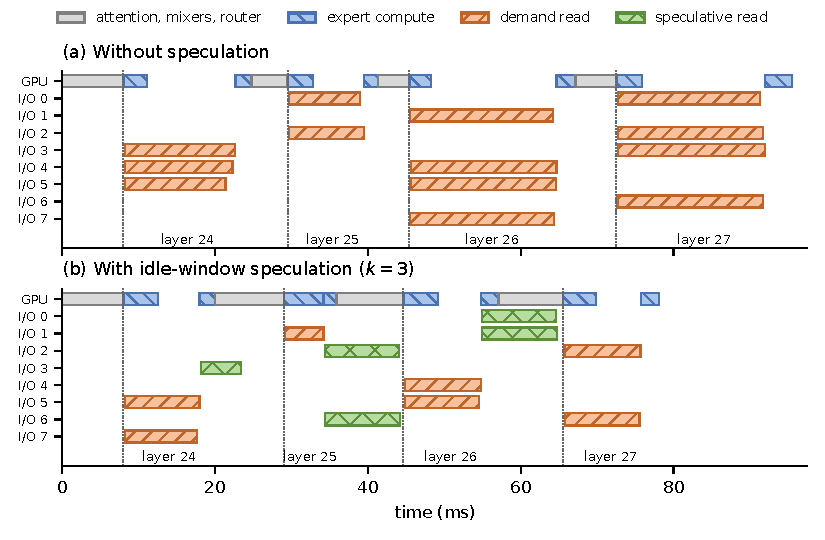
\includegraphics[width=\linewidth]{figures/timeline.pdf}
\caption{Measured timeline of four decode layers with a 5\,GB expert cache. Gray: attention, mixers and router. Blue: expert computation (cached experts first, then the missing ones). Orange: demand reads, one row per I/O thread. Green: speculative reads (\S\ref{sec:spec}). (a) Reads start only after the router of their layer finishes, and the SSD is idle while the GPU works. (b) With idle-window speculation, guesses for the next layer fill this idle time; several experts of each layer are already in memory when the router finishes. Each panel shows the median of three traced tokens. To time GPU work we synchronize after each expert group, which makes a step 2\% (a) and 14\% (b) slower than untraced decoding in the same run.}
\label{fig:timeline}
\end{figure}

This dependency gives a simple cost model. Let $a$ be the time of attention, mixers and router in one layer, $c$ the expert computation time, $m_\ell$ the number of missing experts in layer $\ell$, $b$ the size of one expert and $B$ the SSD bandwidth. A decode step then takes about
\begin{equation}
t_{\text{token}} \;\approx\; \sum_{\ell=1}^{40}\Big(a + c + \frac{m_\ell\, b}{B}\Big).
\label{eq:chain}
\end{equation}
On an idle machine we measured 0.80\,s per token. The compute terms add up to 0.25\,s. With a 49\% hit rate the missing experts total 1.78\,GB; the measured SSD wait was 0.55\,s, which corresponds to 3.2\,GB/s. These numbers roughly add up to the measured step, and they show three ways to make it shorter. The first is fewer misses, which needs a larger cache (\S\ref{sec:replication}). The second is to overlap the reads of a layer with the computation that does not depend on them; inside one layer, that is only the cached experts. The third is to read experts \emph{before} the router asks for them, so that the SSD also works while the GPU computes (\S\ref{sec:spec}).

Section~\ref{sec:parallel-eval} measures each of these options, together with other kinds of parallelism from related systems.

\subsection{Idle-window speculation}
\label{sec:spec}
Equation~\eqref{eq:chain} also shows when the SSD is idle: during $a$ and $c$, while the GPU runs attention and computes experts. In a decode step this idle time adds up to about 0.25\,s, enough to read about 50 experts. Reading the next layer's experts during this time would take reads off the critical path. Prefetching experts is not new \citep{moeoffload,pregated,moeinfinity,promoe,adapmoe}. In particular, \citet{moeoffload} already guess the next layer's experts by applying its gate to the current hidden state, and we use the same predictor. However, prefetching the most likely next-layer experts made decode 5--6\% \emph{slower} in our measurements. Looking at the trace, we suspected two causes, which the ablation in Section~\ref{sec:parallel-eval} later separated:
\begin{itemize}
  \item \textbf{Guesses ran before needed reads.} The engine issued the guesses for layer $\ell+1$ before the misses of layer $\ell$. Both went to the same I/O queue, so every wrong guess delayed a read the token was waiting for.
  \item \textbf{Guesses might pollute the cache.} A guessed expert entered the LRU list as most recently used, so a wrong guess could push out an expert that had been used. The ablation shows that this effect is small at a 5\,GB cache.
\end{itemize}
\emph{Idle-window speculation} addresses both and needs no training or model change. Its essential part is the first: issue guesses only after the demand reads have landed. After the router of layer $\ell$ finishes, the engine also applies the router of layer $\ell+1$ to the current hidden state, using its exact scoring (sqrt-softplus plus bias), and takes the top $k$ experts as guesses. The guesses go to a separate thread that waits until all misses of layer $\ell$ have arrived and only then issues their reads. They therefore run while the GPU computes, in the window where the SSD would otherwise be idle. In addition, a guessed expert is inserted at the \emph{cold} end of the LRU list, the end that is evicted first, similar to low-priority insertion in CPU caches \citep{qureshi2007}. If layer $\ell+1$ uses it, it moves to the hot end; if not, the next guess or miss replaces it before any used expert. A guess never evicts a slot that is pinned or in use by the current request. The change is about 40 lines in the expert store and the MoE block. The ablation in Section~\ref{sec:parallel-eval} shows that the first fix, waiting for the demand reads, provides most of the gain; cold insertion adds a little on top and hurts on its own. Figure~\ref{fig:timeline}b shows the effect: in the same four layers, guessed experts arrive during the GPU's work, and the demand reads that remain are fewer and shorter.

\subsection{Replication: spending memory on the cache}
\label{sec:replication}
Replicating hot experts is the part of EP that transfers most directly. A cluster copies busy experts so that no GPU waits; we keep recently used experts in memory so that no read is needed. Each hit removes one term $b/B$, about 5\,ms, from Equation~\eqref{eq:chain}. We use least-recently-used replacement. On routing traces recorded from the real model, LRU had a higher hit rate than least-frequently-used at the same capacity, and capacity mattered more than the policy: 1.5 times more slots raised the hit rate from 0.38 to 0.47.

Because cache size drives decode speed, the rest of the design tries to save memory:
\begin{itemize}
  \item Dense FP8 weights convert to MXFP8 without loss (Section~\ref{sec:impl}), so we never keep a higher-precision copy.
  \item Expert reads skip the page cache, so the same expert is never stored twice.
  \item Speculative reads enter the cache cold (\S\ref{sec:spec}), and speculative decoding is off by default, so neither pushes useful experts out.
\end{itemize}
The cache size is set at start-up from the memory that is free at that moment, minus a 4\,GB margin, and at least 9\,GB always stay free for macOS. With less than that the system starts swapping and decode slows down sharply. On an idle 24\,GB machine this gives 5--6\,GB of expert slots.

We also provide an optional approximation based on the same idea. If a missing expert carries less than 8\% of a token's routing weight, the engine skips it and saves the read. It lowers top-1 agreement with the API on open-ended text by 2.4 points. We did not measure its speed effect in an interleaved test, so we report no speed-up for it, and it is off by default.
